\subsection{Importance of learning self-defined categories}
Nowadays, more and more companies provide individual service for their clients. Personalized recommendation system has been widely used in many electronic commerce, such as Amazon and eBay. The requirement of personalized service is growing every year. Personalized system means it is possible to handle the variance of the request from individuals. For image recognition, many interesting applications have been proposed. However, unlike other personalized system, it is difficult to train personalized recognition system for individuals. There could be enormous variances of one object and it is always difficult for a model to capture these variances.

Even though, the state-of-the-art recognition system can do as well as a human, its great success is achieved based on the fact that millions of labeled training images are used for training. Selecting large amount of images for the new categories is always a tedious job.
Moreover, an important property of self-defined category images is that the source of the data is inherently scarce. Therefore, it is not possible to obtain abundant training data. For example, users of Google's im2calories can track their nutrition of every meal by taking a pictures of their foods via image recognition techniques. The system firstly check the category of each food item and find their nutritions in the database. However, the existing model can only recognize the general food categories which means it is not possible for a user to track the nutrition of his/her daily home-made meals. These home-made foods can be similar to some existing food categories (home-made veggie burger can be similar to burger in McDonald), but they may have different nutritions. This scenario can be applied to learning any exclusive category in our life. Therefore, a model that can learn these self-defined categories can be important.

\begin{figure}
	\centering
	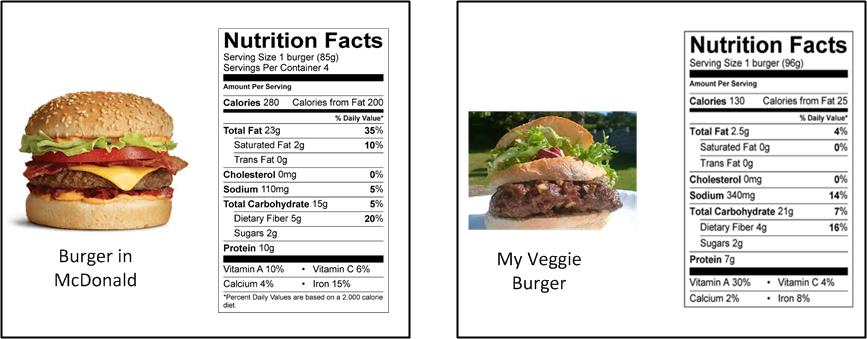
\includegraphics[scale=.6]{introduction/fig/scenario.jpg}
	\caption{Different nutrition facts between the burgers in McDonald and home-made.}\label{fig:intro:scenario}
\end{figure}

Our human is good at learning the new objects. For our human, all the information acquired is stored in our memory. These information are organized according to the properties. When we see a new concept, we don't treat it isolated, but connect it to certain previous knowledge we stored in our memory. By comparing a new concept with the organized information in our memory, we can capture the property of a new concept effectively. When referring to visual tasks, several examples can be given to show this cognitive ability. For instance, when we describe the animal "zebra", we would probably say that: zebra is a horse with while and black striped coats. People who never see a zebra could instantly have a rough idea of a zebra. 

This means to learn a new category effectively, we should be able to make use of the gained knowledge instead of learn it from scratch. This process is commonly refer to as transfer learning. Traditional machine learning methods work under the common assumption: training data and testing data are drawn from the same feature space and same distribution. When considering adding classifying the data from the new categories, the distribution of the data changes and a new model should be rebuilt from newly collected data.Those data from the original distribution is called source data and data from the new distribution is called target data. Transfer learning is used to utilize the source knowledge from the source data to help training the new model to classify the target data. 

%\hl{We can keep learning new categories throughout our whole life and become more proficient as we learn more. Human doesn't need large amount of training data to adapt a new object. In most scessnario, we can still recognize the new object well by a few examples, e.g. taking a glancing at the object. This indicates that it is possible for a recognition model to adapt by just a few training examples from the new categories.}
In this thesis, we try to use transfer learning approaches to solve the problem of learning self-defined categories. We can find many examples in knowledge engineering where transfer learning does benefit the learning process \cite{pan2010survey}. This implies that, by leveraging the learned knowledge properly, we can learn the self-defined categories with a few examples. 
In this thesis, we also assume that the self-defined categories are not isolated and similar to certain existed categories. Therefore, we can use leverage the knowledge from those existed categories to help us learn the self-defined categories. Then, we split the self-defined categories into two groups according to their relationship to the exited categories: 
\begin{itemize}
	\item One source category, a category that is very similar to one existed category. For example, my veggie burger can be very similar to general burger and less similar to other categories.
	\item Multi-source category, a category that doesn't have an explicit similarity to one category but share some properties with several existed categories (see figure \ref{fig:intro:multi} for instance).
\end{itemize} 
Due to different properties of these two groups, we should design different strategies to adapt them.

\begin{figure}
	\centering
	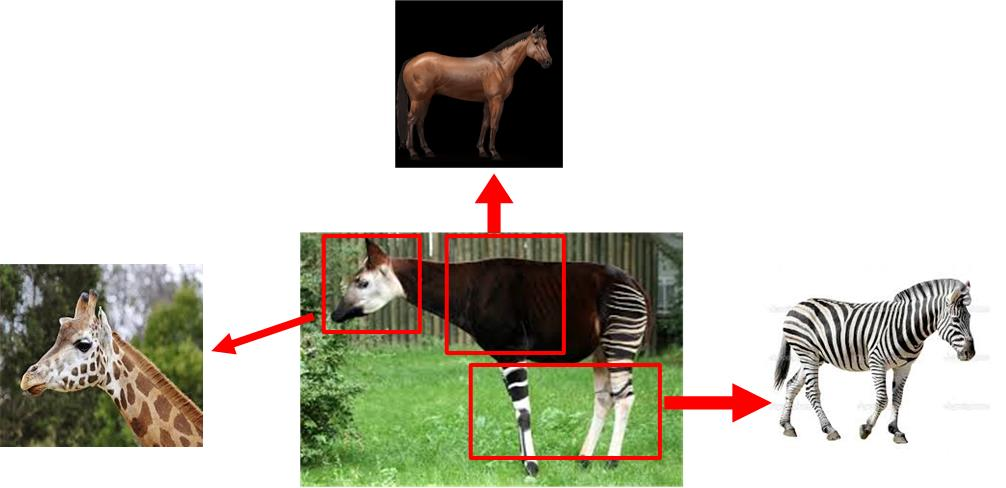
\includegraphics[scale=.6]{introduction/fig/multiple.jpg}
	\caption{Multi-source category case: an okapi can be roughly described as the combination of a body of a horse, legs of the zebra and a head of giraffe.}\label{fig:intro:multi}
\end{figure}

\subsection{Assumption of the source knowledge}
In transfer learning, the source knowledge can be presented in two different ways \cite{pan2010survey}: 
\begin{itemize}
	\item Instance transfer learning. Even though the source data can not be re-used directly, certain part of the data can be used incorporating with a few labeled target data to train the model.
	\item Parameter transfer learning. Instead of utilizing the source data, parameter transfer learning approaches re-use the parameters of the model trained from source data (called the source model). 
\end{itemize}

In this thesis, we try to explore a method to learn self-defined categories via the parameter transfer learning approach and try to utilizing the source data in a hard way, by assuming that the source data is access prohibited and we can only access the trained model from the source data.
This assumption is made based on the following two facts: (1) In some situations, we may not be able to access the source data and only the model trained from the source data is available. There are many credential datasets. Therefore, it is not always possible to fully access the source data. (2) The source data could be very large and it could be tedious to determine which part of the data could benefit the transfer learning. On the other hand, the trained model from the source data can be as informative as the source data itself. For example, the information extracted from the support vectors (SVs) of a SVM model trained from a dataset could be as much as the information of the whole dataset. Some results from recent work also show that it is possible to obtain a good model by even just utilize the source models and learn new categories from a few examples \cite{fei2006one} \cite{tommasi2010safety} \cite{tommasi2014learning}.

In this section, we discuss the scenario of the learning self-defined category problem. We conclude that learning self-defined categories can be achieved by transfer learning. We also make an assumption that we can only access the model trained from the source data and the source data itself is prohibited. \hl{In the next section, we discuss the challenges of our problem.}

%In this thesis, we propose a novel transfer learning method, called \textbf{SMITLe} (\textbf{S}afety \textbf{M}ulticlass \textbf{I}ncremental \textbf{T}ransfer \textbf{Le}arning) that is able to learn new categories from a few examples.